\section{New Method}
\subsection{Problem summary}
For multi-core chip in dark silicon era, cores on the chip can not be all turned on at the same time due to the
thermal constraint. In order to make full use of the chip resources, we need to decide the number of active cores as
well as the corresponding specific distribution that lead to maximum chip performance. Usually, we can use the frequency
for performance measurement. Which should be noticed is that, active cores on the chip may not run at its maximum supply voltage
and frequency, instead, it can be applied with Dynamic Voltage and Frequency Scaling(DVFS).
\subsection{Relation between voltage and frequency}
Actually, the operating frequency of core is decided by its supply voltage, following equation can be used to shows the dependency
of frequency on voltage:
\begin{equation}\label{v_and_f}
f \propto (V-V_{th})^{\gamma}/V.
\end{equation}
Where $V$ is the transistor's supply, $V_{th}$ is the threshold voltage, $f$ is the operating frequency and the exponent
$\gamma$ is an experimentally derived constant decided by the process of chip.

With the above equation, we can further develop a linear equation relating frequency and voltage. First, we normalize the
voltage and frequency to their maximum values as $V_{norm}=V/V_{max}$ and $f_{norm}=f/f_{max}$, then we can approximate a linear
relationship with following equation:
\begin{equation}\label{V_and_f_linear}
V_{norm} = \beta_1+\beta_2 \cdot f_{norm},
\end{equation}
where $bata_1=V_{th}/V_{max}$ and $beta_2=1-beta_1$, value of $beta_1$ can be considered to be around \SI{0.4} for typical process\cite{Taylor:MICRO'13}.
From this equation, we can recognize that the frequency will have to be reduced to zero when supply voltage is reduced to $V_{th}$,
which surely becomes the lower bound of voltage in DVFS operation.
\subsection{Problem formulation}
Power of cores on the chip can be divided to be dynamic power $p_d$ and static power $p_s$, where
\begin{equation}\label{pd_ps}
p_d=A C V^2 f,\\
p_s=V I_{leak},
\end{equation}
where A is the fraction of gates actively switching and C is the total capacitance load of all gates, $I_{leak}$ is the leakage current of
core.
Assume the dynamic power and static power with no DVFS of cores are $P_{d_0}=[p_{d_{0_1}},p_{d_{0_2}},\ldots,p_{d_{0_l}}]^ \mathrm{ T }$
$P_{s_0}=[p_{s_{0_1}},p_{s_{0_2}},\ldots,p_{s_{0_l}}]^ \mathrm{ T }$, where $p_{d_{0_i}}$ and $p_{s_{0_i}}$ are dynamic power and static power
of $i-th$ core respectively. When DVFS is performed, assume the voltage scaling ratio of $i-th$ core is $\alpha_i$, then according to \ref{V_and_f_linear},
the corresponding scaling ratio of frequency is $\lambda_i=\alpha_i \theta_i$, so the scaling ratio of dynamic power is $\alpha \lambda$ according
to \ref{pd_ps}. For static power, the effect of voltage and frequency scaling is much less than dynamic power, and its scaling ratio can be considered
as $\alpha_i^\kappa$, where $\kappa$ is a process-related constant, for simplicity sake, we can assume $\kappa=1$, in other words, we can ignore
the effect of leakage's dependency on voltage. Also, we use Boolean variable $\xi_i \in \left\{0,1\right\}$ to represent the $i-th$ core is active or
not: $xi_i=0$ represents inactive and $xi_i=1$ represents active situation.

As mentioned before, we could use operating frequency to measure the performance of cores, and DVFS operation determine the real frequency, our
optimization goal can be expressed as $\sum_{i=1}^l \xi_i \theta_i f_{max_i}$. Because the main limit of chip performance is the cooling capacity,
so we can express the steady temperature use thermal model and let it under the temperature threshold:
$G^{-1} B \xi \left( \Lambda P_{d_0} + \alpha P_{s_0} \right) \prec T_{max}$.
Where $\Lambda \in \mathbb{R}^{l \times l} $, $\alpha \in \mathbb{R}^{l \times l} $ and $\xi \in \mathbb{R}^{l \times l}$ are all diagonal matrices,
their $i-th$ diagonal element are $\lambda_i$, $\alpha_i$ and $\xi_i$ respectively. $\prec$ is vector inequality, for m-dimensional vector, $u$ and $v$,
$u \prec v$ represents that $u_i < v_i$ for $i = 1$,$2$,$\ldots$,$m$.

Finally, we can express the whole optimization problem using following equation:
\begin{align*}
&\max\,\, \sum_{i=1}^l \xi_i \theta_i f_{max_i}\\
&s.t.\quad
\begin{cases}
G^{-1} B \xi \left( \Lambda P_{d_0}+ \alpha P_{s_0} \right) \prec T_{max}\\
\alpha_i \in \left(0,1\right], &i=1,2,\ldots,l  \\
\xi_i \in \left\{0,1\right\}, &i=1,2,\ldots,l
\end{cases}
\end{align*}
Solving this optimization problem, we can get the best $\alpha_i$ and $\xi_i$��then get best number and distribution of active cores using the number of
non-zero elements in $\xi$, and also get the power budget of cores with the value of $\alpha_i$.
\subsection{use greedy algorithm to solve the optimization problem}
A basic solution for the above equation is to traverse all possible values of $\lambda_i$, $\alpha_i$ and $\xi_i$ of all cores under the thermal limit,
and choose the values that result in maximum total performance. However, although this method can allow us to find the optimal solution, the time consumption
is unacceptable, with number of cores increasing, this method will soon be useless.

To reduce the time cost and find a acceptable approximate solution, we propose a greedy algorithm to replace the ergodic method.
For a chip with $m$ total cores, the basic idea of our proposed greedy algorithm can be described as follow: first we find a sub-optimal distribution for each active
core number from \SI{1} to $m$, together with the total chip performance, then compare the chip performance with different number of active cores and get
the best active-core number which result in best chip performance, as well as the corresponding distribution.

The details of finding sub-optional for certain active-core number $m$ is as follow: we first find the optimal solution for only one active core. Then, we keep
the first active core position determined by first step, and find the optimal solution of two cores, with the second active core position determined. Such strategy
will be iteratively processed for $m$ steps, and finally we can arrive at a sub-optimal solution for $m$ active cores.

Naturally, the first active position affect the subsequent active positions a lot, especially when the total active-core
number $m$ is small. That is because the first active core will determine the second position and thus the 3rd one, ...
untill the last one. A natural idea to relieve this is to add more choices for the starting position instead of only the
optimal one, then start from different core position to find the sub-optimal distribution for the certain active-core
number $m$, at last,  compare the total performance resluted by different beginning position and finally determine the
best distribution for active cores.
%\subsubsection{ Application of symmetry for initial active core search}
Take the actual situation as a reference, we can make a reasonable assumption that the cores on the chip are distributed as square form. Cores distributed in
this particular distribution form has strong symmetry, which enable us to decrease the choices of the first active core
position without losing completeness, and thus save a lot time to find the sub-optional distrubution for certain
active-core number.

As shown in Fig.~\ref{fig:symmetry}, we can take a 16-core chip as example, which has only three different positions when determine
the first active core when the symmetry of cores are considered. And it is easy to realize that for a chip with $n
\times n$ cores, the different number of positions for first active core is just $(\bar{n}^2+\bar{n})/2$, where
$\bar{n}$=$\lceil n/2 \rceil$.
\subsection{Temporary experimental result}
We test our greedy algorithm on a chip with $4 \times 4$ cores and get some acceptable experimental results as we
excepted. Fig.~\ref{fig:performance_compare} shows the comparison of our new method and the basic ergodic method in finding the maximum total
performance when a certain number of active cores is given. It is clear that the result of our new method is nearly the
same as that of the time consuming ergodic method. We also show the distribution given by these two methods when the
active-core number is \SI{10}, which result in the maximum total performance for this 16-core chip just as shown in
Fig.~\ref{fig:dis_compare}, as we can see, the two distribution are just the same because of the symmetry of cores. 
As for time cost, the ergodic method takes \SI{13.507}s to go through all possible active-core numbers and distributions 
while our greedy method only cost \SI{0.056}s. 

\begin{figure}
\centering
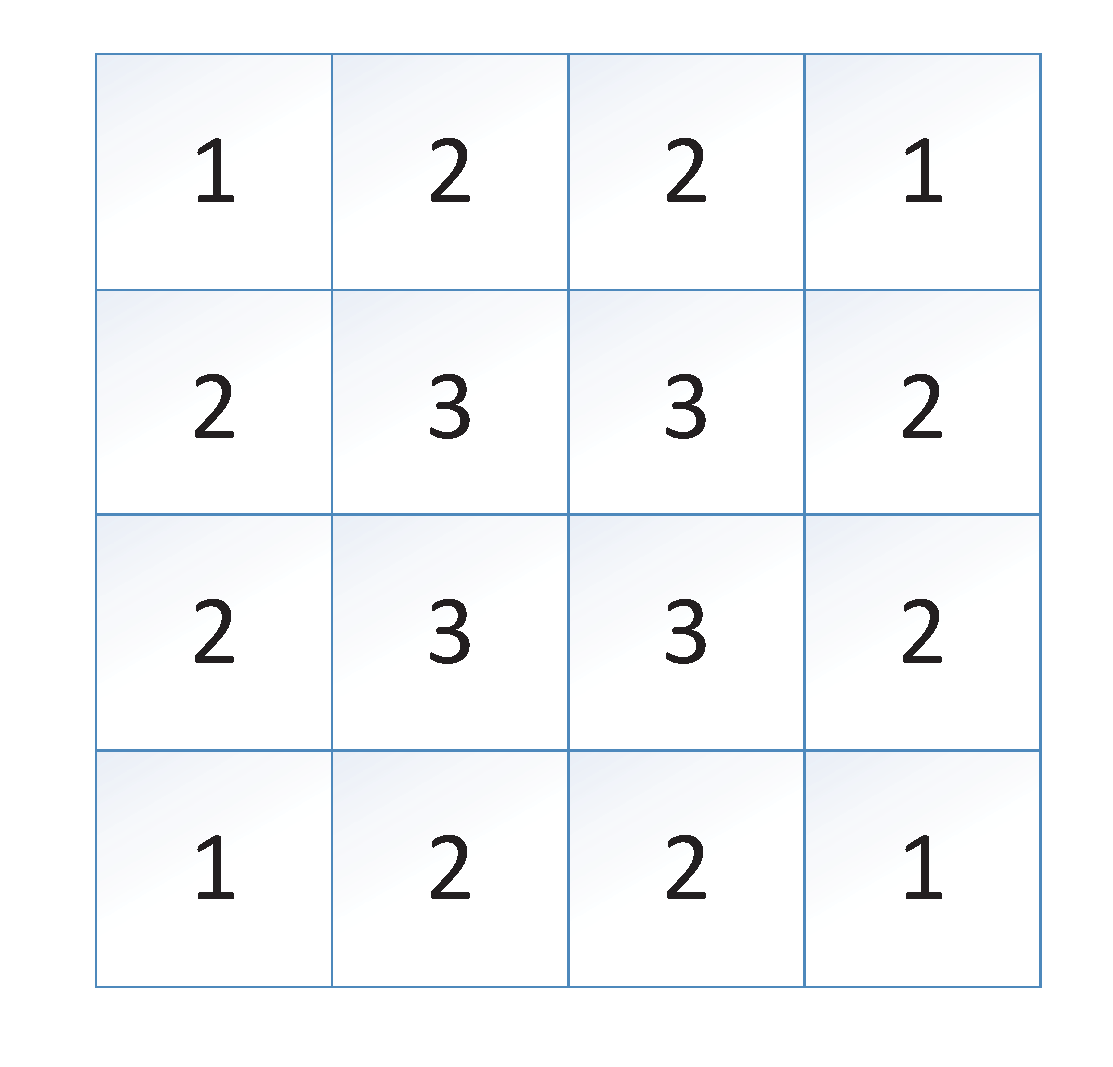
\includegraphics[width=0.7\columnwidth]{fig/symmetry.eps}
\caption{An example of symmetry of a chip of $4 \times 4$ cores, cores marked with same number can be considered to be equivalent
when determine the first active core.
}
\label{fig:symmetry}
\end{figure}

\begin{figure}
\centering
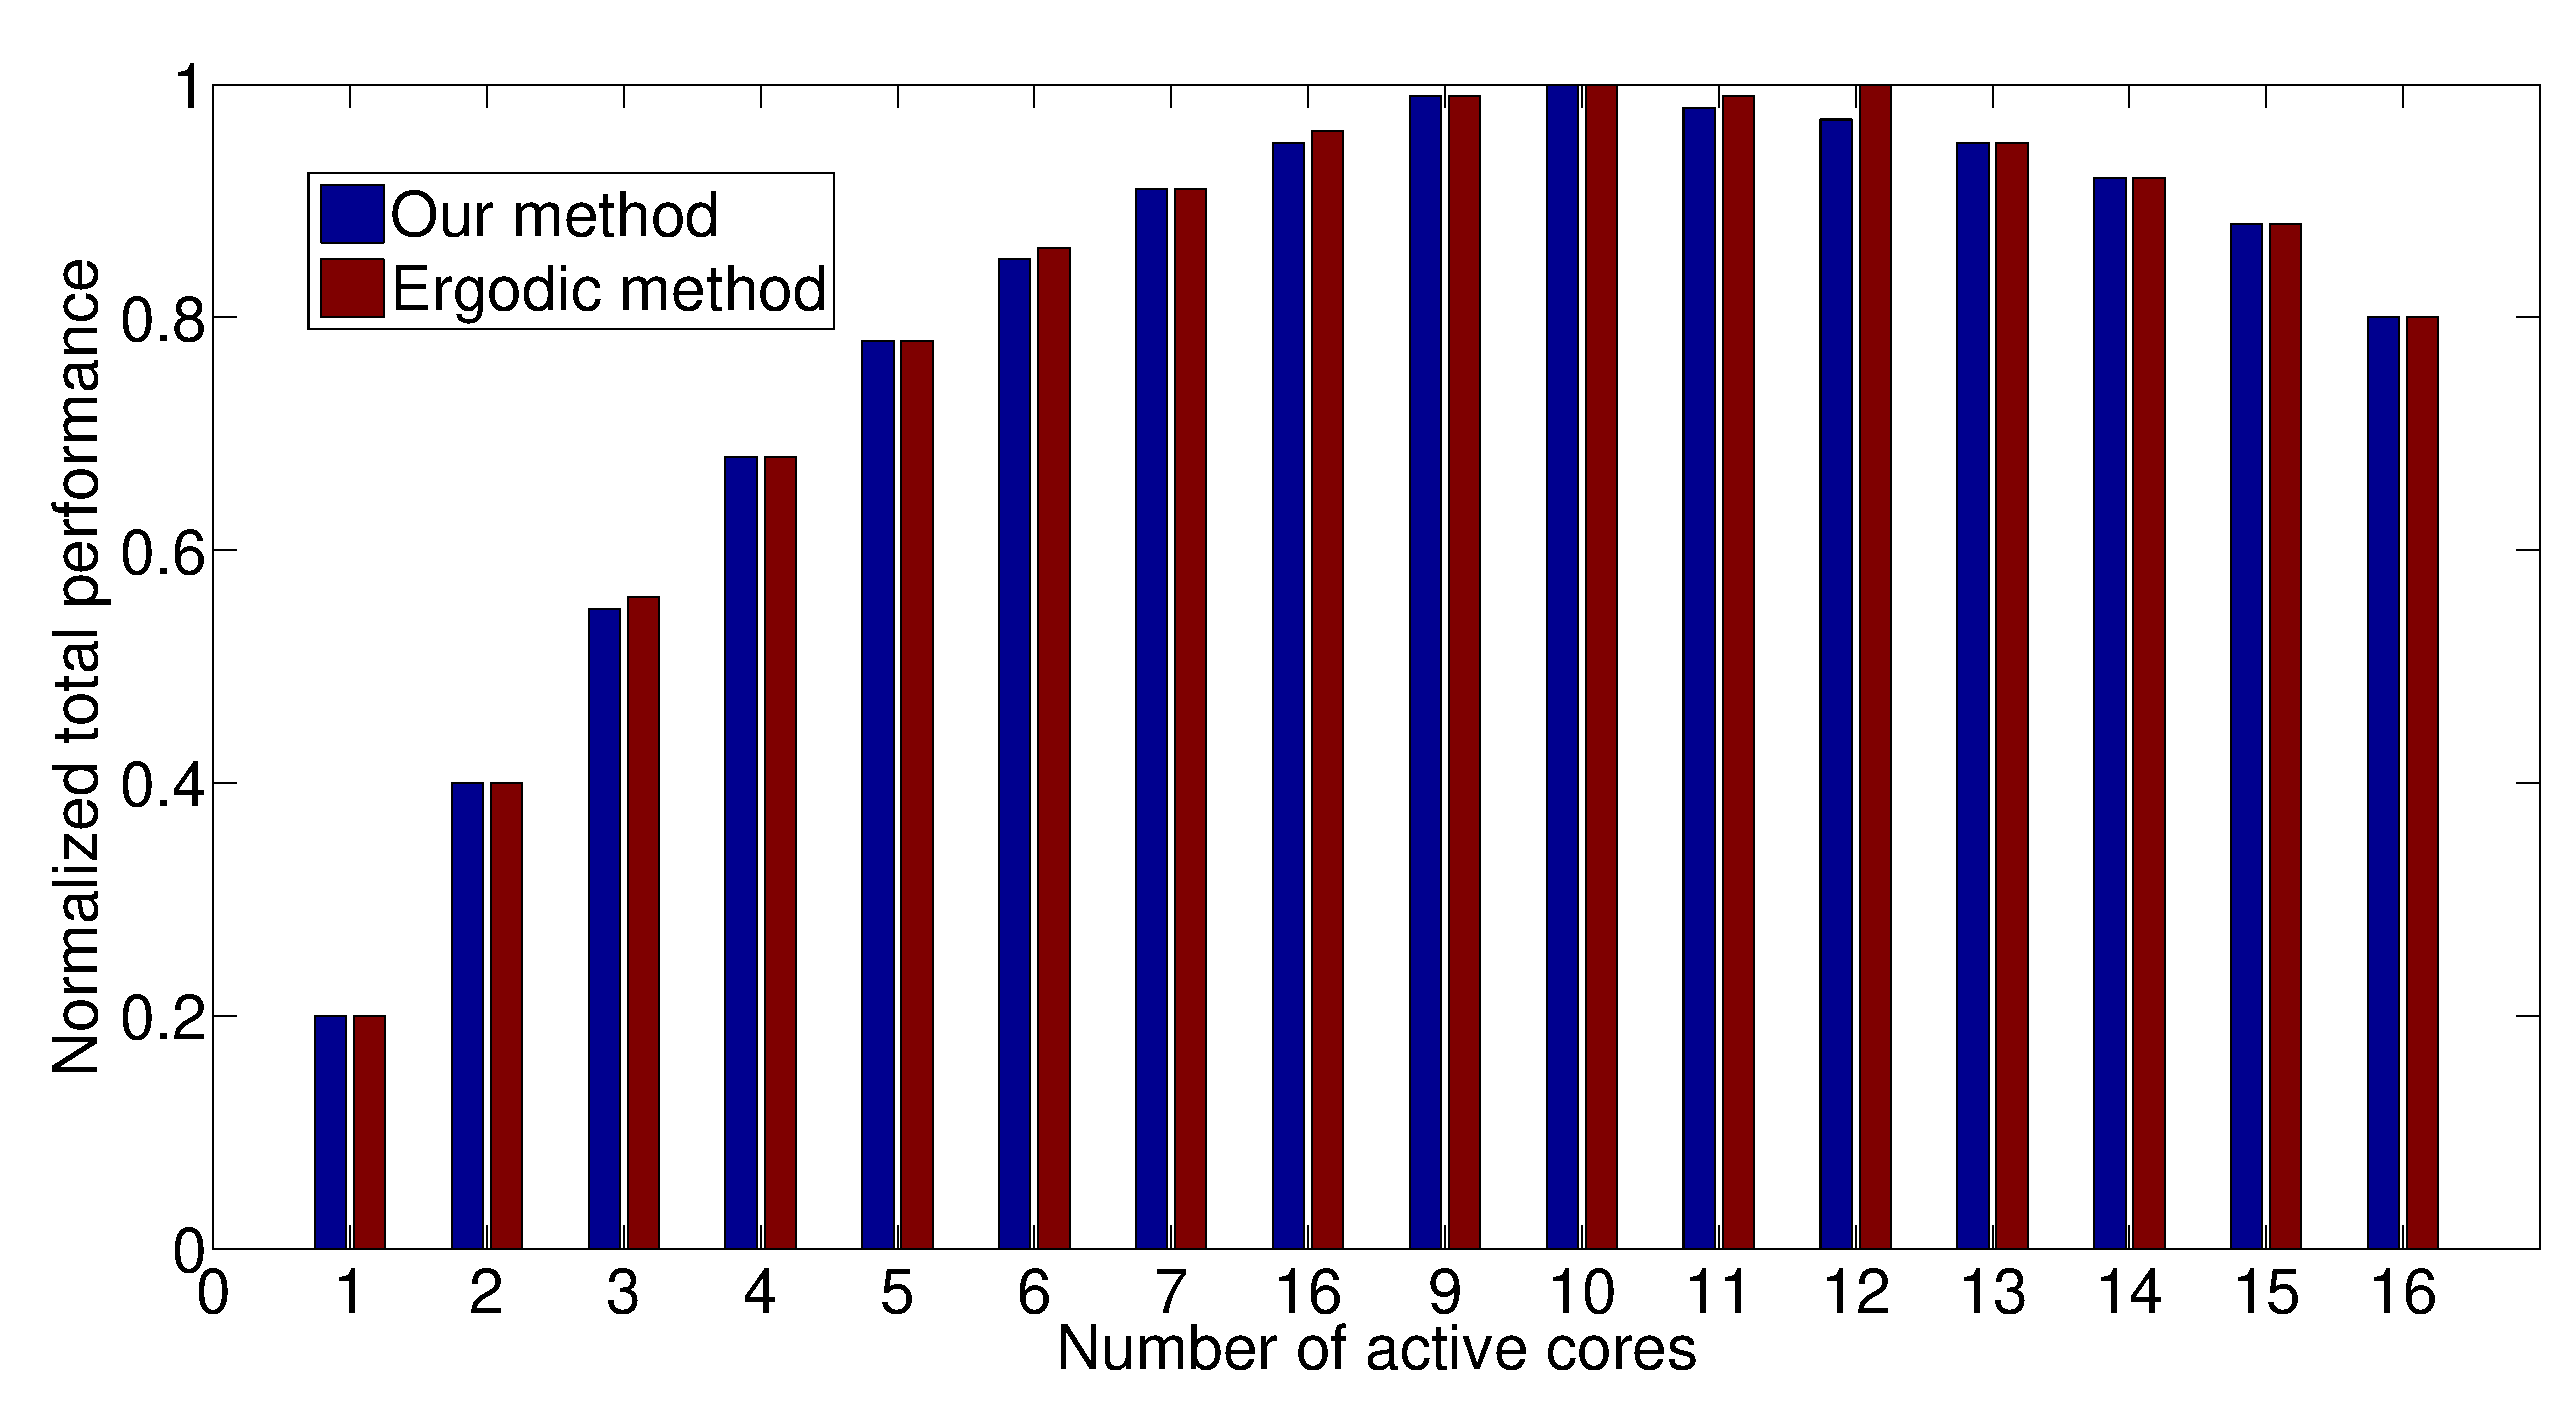
\includegraphics[width=0.9\columnwidth]{fig/performance_compare.eps}
\caption{Comparison of Normalized total performance given by two methods for different number of active cores.}
\label{fig:performance_compare}
\end{figure}

\begin{figure}
\centering

\subfigure[Best distribution given by ergodic method.]{
\label{fig:dis_compare_erg}
%\begin{minipage}[b]{0.4\textwidth}
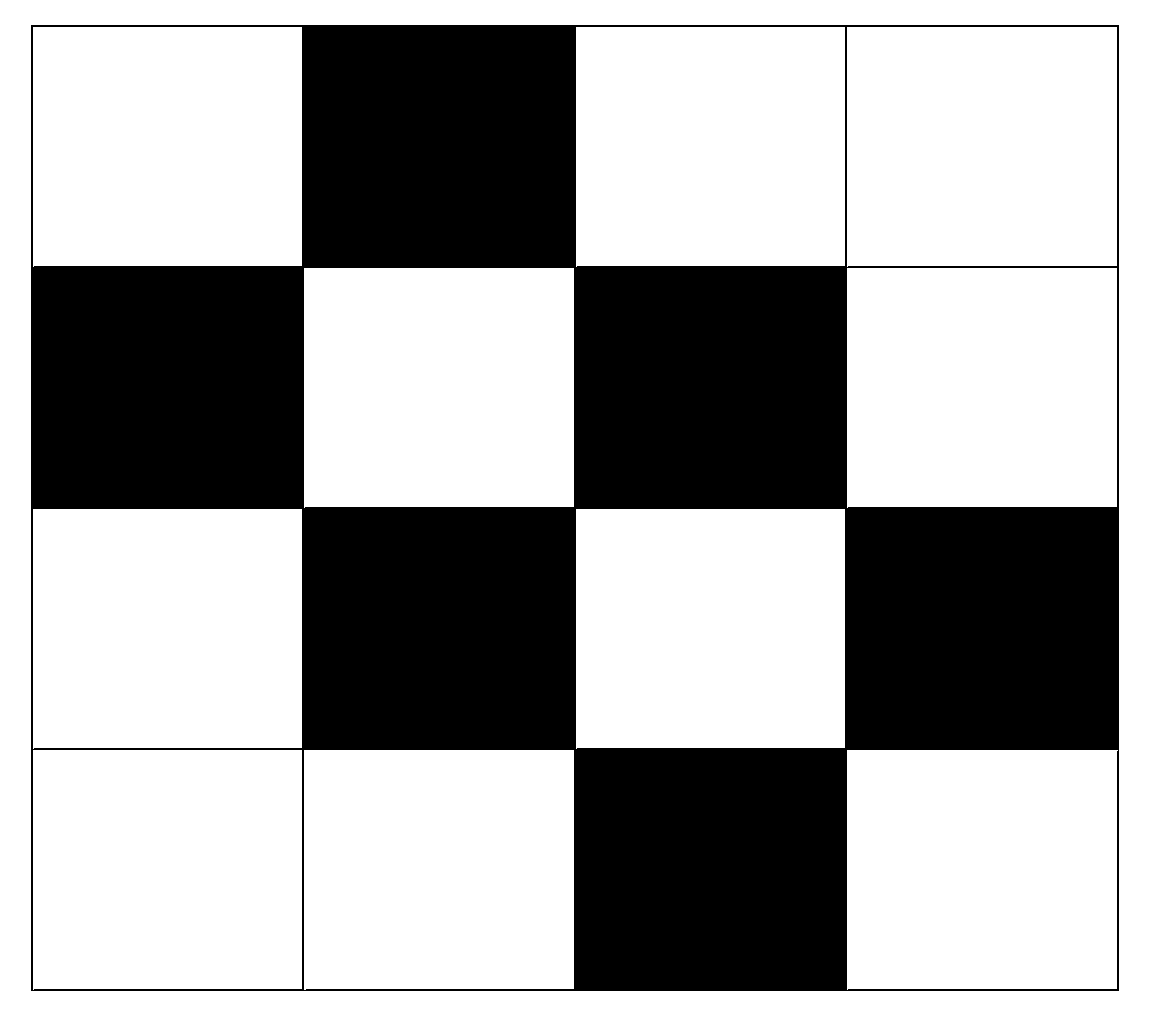
\includegraphics[width=0.6\columnwidth]{fig/dis_erg.eps}
%\end{minipage}
}
\subfigure[Best distribution given by our new method.]{
\label{fig:dis_compare_new}
%\begin{minipage}[b]{0.4\textwidth}
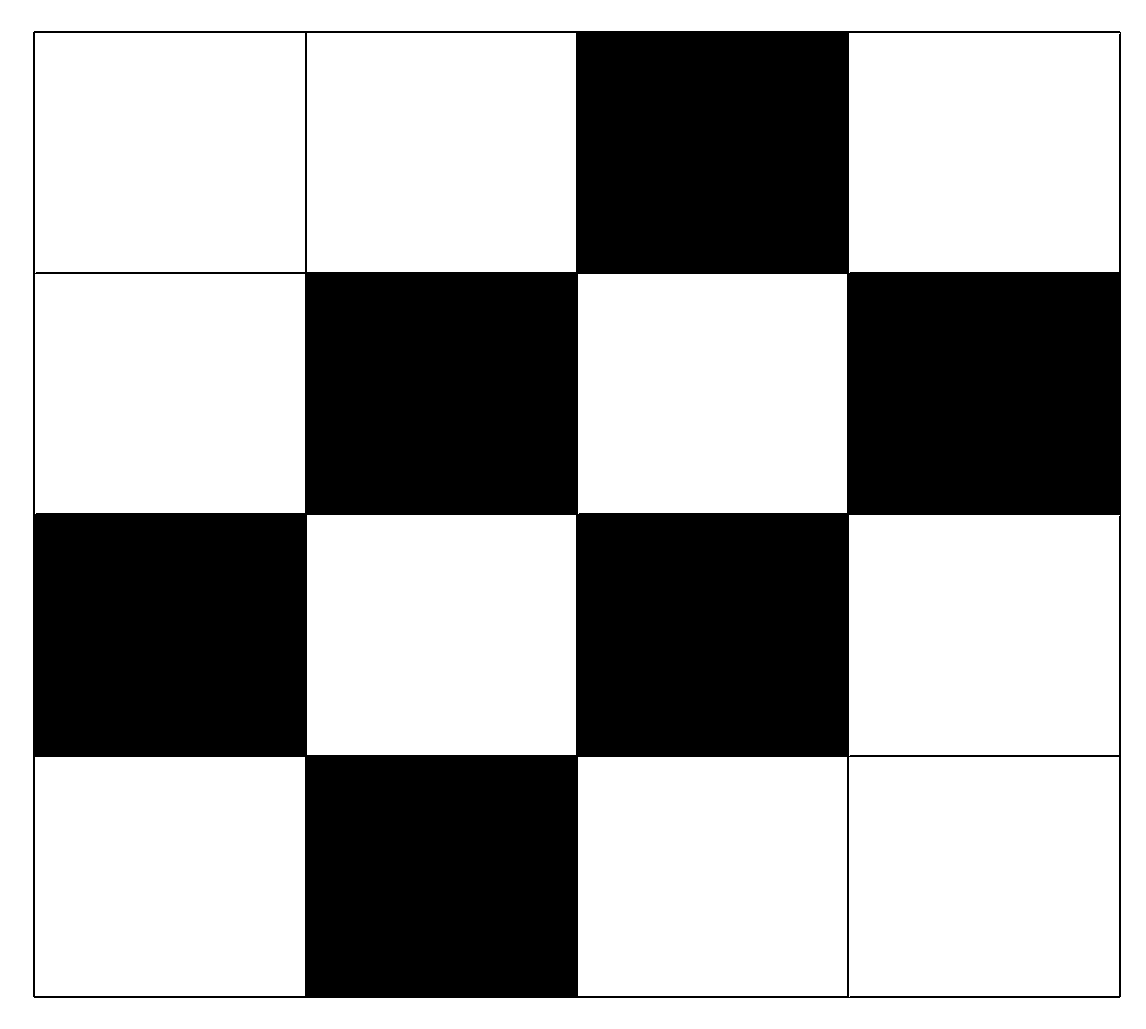
\includegraphics[width=0.6\columnwidth]{fig/dis_new.eps}
%\end{minipage}
}

\caption{Comparison of distributions given by two methods when the active-core number is set to be 10.}
\label{fig:dis_compare}
\end{figure}







